%!TeX root=../pridetop.tex
\chapter[Chapter \thechapter]{}
	
	
\begin{figure}[t!]
\centering
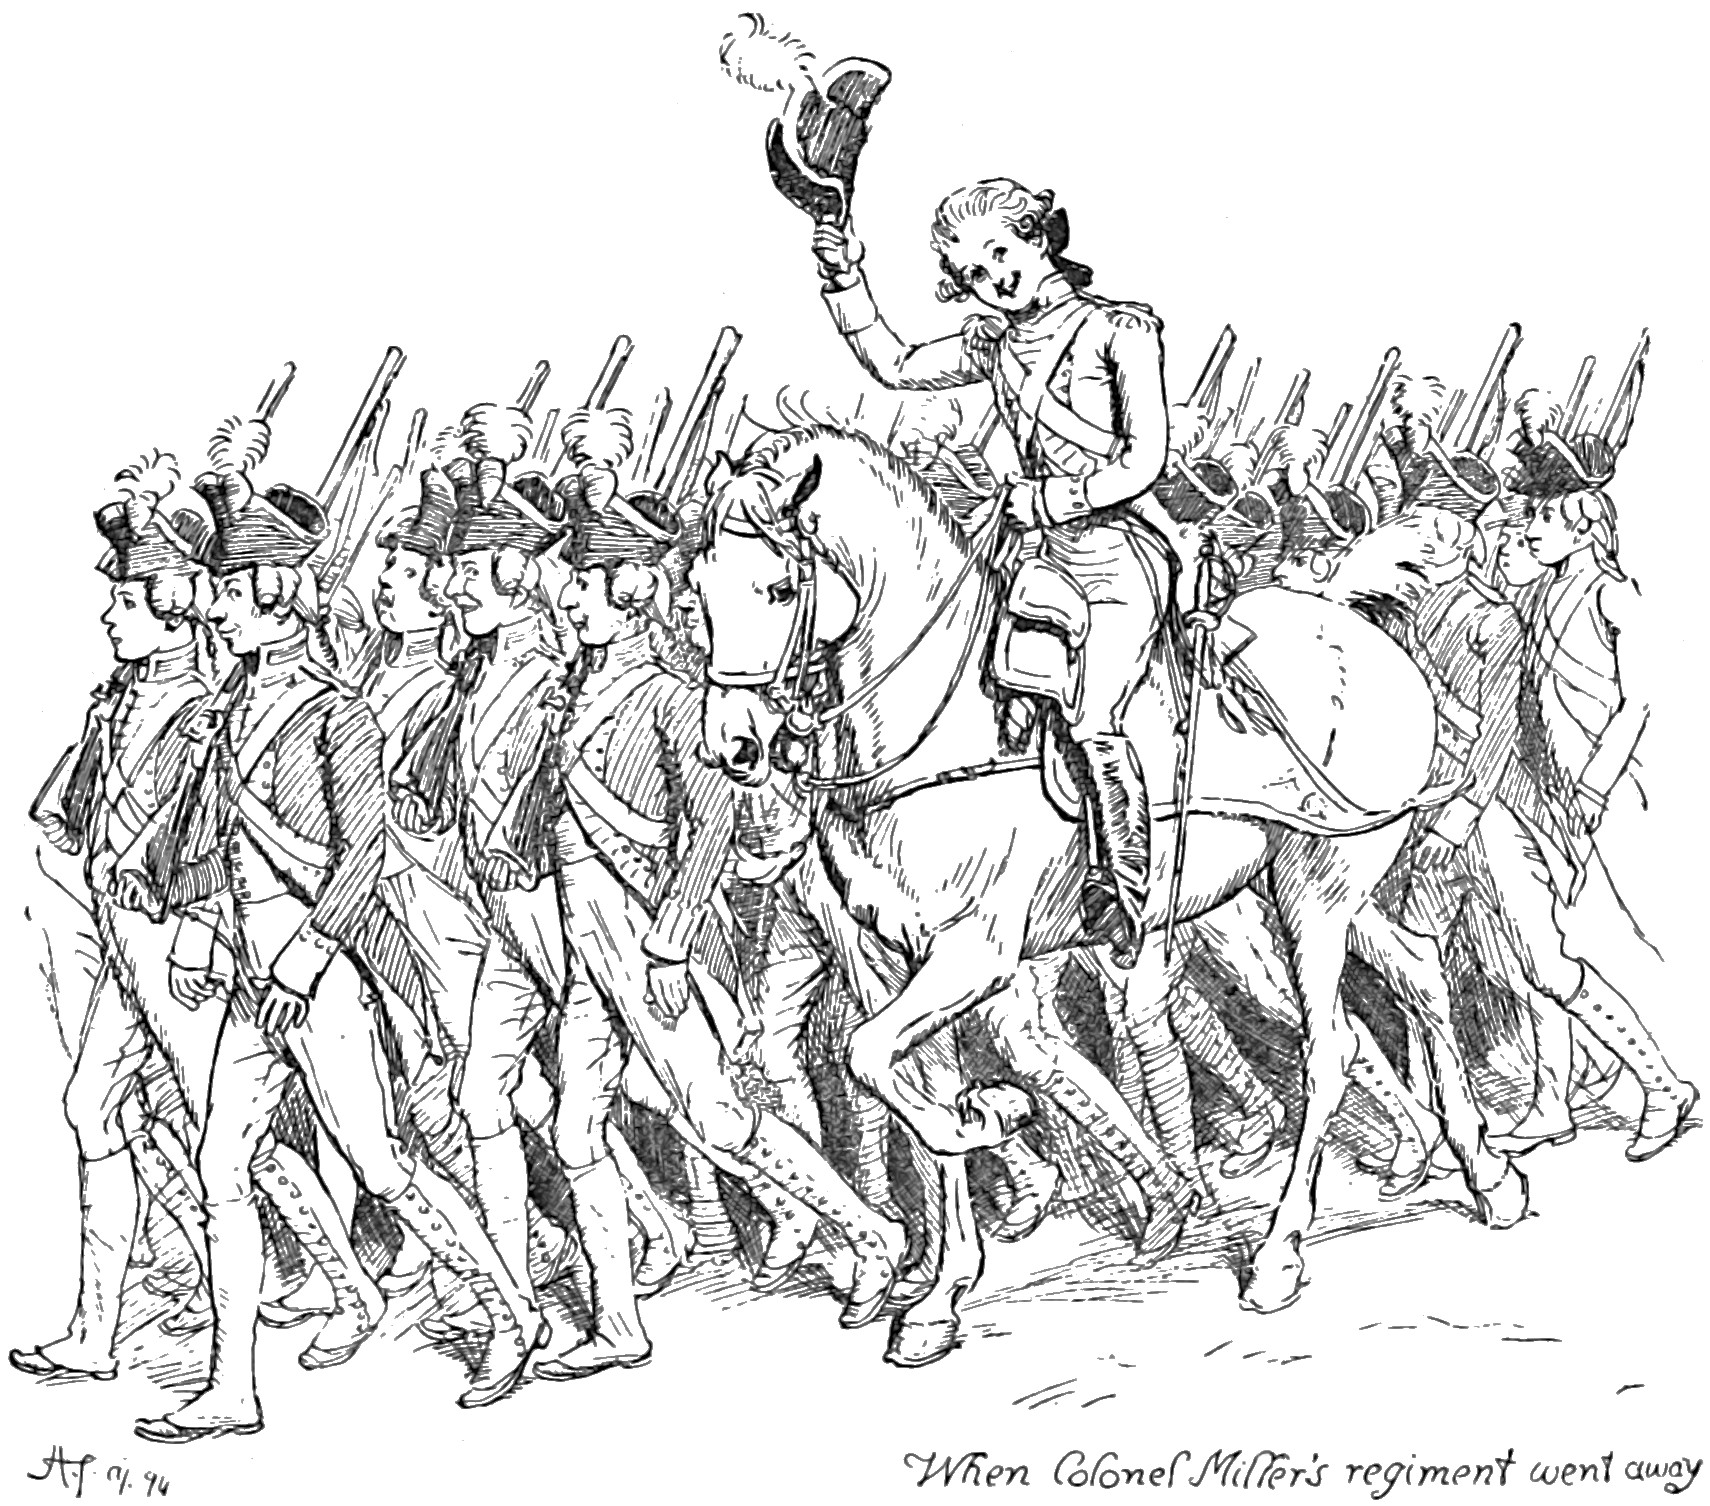
\includegraphics[width=\linewidth]{41top}
\captionlistentry{When Colonel Miller's regiment went away}
\end{figure}


\lettrine[lines=6,image=true]{initials/chap41t}{he}  first week of their return was soon gone. The second began. It was the last of the regiment's stay in Meryton, and all the young ladies in the neighbourhood were drooping apace. The dejection was almost universal. The elder Miss Bennets alone were still able to eat, drink, and sleep, and pursue the usual course of their employments. Very frequently were they reproached for this insensibility by Kitty and Lydia, whose own misery was extreme, and who could not comprehend such hard-heartedness in any of the family.

»Good Heaven! What is to become of us? What are we to do?« would they often exclaim in the bitterness of woe. »How can you be smiling so, Lizzy?«

Their affectionate mother shared all their grief; she remembered what she had herself endured on a similar occasion five-and-twenty years ago.

»I am sure,« said she, »I cried for two days together when Colonel Miller's regiment went away. I thought I should have broke my heart.«

»I am sure I shall break \textit{mine},« said Lydia.

»If one could but go to Brighton!« observed Mrs Bennet.

»Oh yes!—if one could but go to Brighton! But papa is so disagreeable.«

»A little sea-bathing would set me up for ever.«

»And my aunt Philips is sure it would do \textit{me} a great deal of good,« added Kitty.

Such were the kind of lamentations resounding perpetually through Longbourn House. Elizabeth tried to be diverted by them; but all sense of pleasure was lost in shame. She felt anew the justice of Mr Darcy's objections; and never had she before been so much disposed to pardon his interference in the views of his friend.

But the gloom of Lydia's prospect was shortly cleared away; for she received an invitation from Mrs Forster, the wife of the colonel of the regiment, to accompany her to Brighton. This invaluable friend was a very young woman, and very lately married. A resemblance in good-humour and good spirits had recommended her and Lydia to each other, and out of their \textit{three} months' acquaintance they had been intimate \textit{two}.

The rapture of Lydia on this occasion, her adoration of Mrs Forster, the delight of Mrs Bennet, and the mortification of Kitty, are scarcely to be described. Wholly inattentive to her sister's feelings, Lydia flew about the house in restless ecstasy, calling for everyone's congratulations, and laughing and talking with more violence than ever; whilst the luckless Kitty continued in the parlour repining at her fate in terms as unreasonable as her accent was peevish.

»I cannot see why Mrs Forster should not ask \textit{me} as well as Lydia,« said she, »though I am \textit{not} her particular friend. I have just as much right to be asked as she has, and more too, for I am two years older.«

In vain did Elizabeth attempt to make her reasonable, and Jane to make her resigned. As for Elizabeth herself, this invitation was so far from exciting in her the same feelings as in her mother and Lydia, that she considered it as the death-warrant of all possibility of common sense for the latter; and detestable as such a step must make her, were it known, she could not help secretly advising her father not to let her go. She represented to him all the improprieties of Lydia's general behaviour, the little advantage she could derive from the friendship of such a woman as Mrs Forster, and the probability of her being yet more imprudent with such a companion at Brighton, where the temptations must be greater than at home. He heard her attentively, and then said,—

»Lydia will never be easy till she has exposed herself in some public place or other, and we can never expect her to do it with so little expense or inconvenience to her family as under the present circumstances.«

»If you were aware,« said Elizabeth, »of the very great disadvantage to us all, which must arise from the public notice of Lydia's unguarded and imprudent manner, nay, which has already arisen from it, I am sure you would judge differently in the affair.«

»Already arisen!« repeated Mr Bennet. »What! has she frightened away some of your lovers? Poor little Lizzy! But do not be cast down. Such squeamish youths as cannot bear to be connected with a little absurdity are not worth a regret. Come, let me see the list of the pitiful fellows who have been kept aloof by Lydia's folly.«

»Indeed, you are mistaken. I have no such injuries to resent. It is not of peculiar, but of general evils, which I am now complaining. Our importance, our respectability in the world, must be affected by the wild volatility, the assurance and disdain of all restraint which mark Lydia's character. Excuse me,—for I must speak plainly. If you, my dear father, will not take the trouble of checking her exuberant spirits, and of teaching her that her present pursuits are not to be the business of her life, she will soon be beyond the reach of amendment. Her character will be fixed; and she will, at sixteen, be the most determined flirt that ever made herself and her family ridiculous;—a flirt, too, in the worst and meanest degree of flirtation; without any attraction beyond youth and a tolerable person; and, from the ignorance and emptiness of her mind, wholly unable to ward off any portion of that universal contempt which her rage for admiration will excite. In this danger Kitty is also comprehended. She will follow wherever Lydia leads. Vain, ignorant, idle, and absolutely uncontrolled! Oh, my dear father, can you suppose it possible that they will not be censured and despised wherever they are known, and that their sisters will not be often involved in the disgrace?«

Mr Bennet saw that her whole heart was in the subject; and, affectionately taking her hand, said, in reply,—

»Do not make yourself uneasy, my love. Wherever you and Jane are known, you must be respected and valued; and you will not appear to less advantage for having a couple of—or I may say, three—very silly sisters. We shall have no peace at Longbourn if Lydia does not go to Brighton. Let her go, then. Colonel Forster is a sensible man, and will keep her out of any real mischief; and she is luckily too poor to be an object of prey to anybody. At Brighton she will be of less importance even as a common flirt than she has been here. The officers will find women better worth their notice. Let us hope, therefore, that her being there may teach her her own insignificance. At any rate, she cannot grow many degrees worse, without authorizing us to lock her up for the rest of her life.«

With this answer Elizabeth was forced to be content; but her own opinion continued the same, and she left him disappointed and sorry. It was not in her nature, however, to increase her vexations by dwelling on them. She was confident of having performed her duty; and to fret over unavoidable evils, or augment them by anxiety, was no part of her disposition.

Had Lydia and her mother known the substance of her conference with her father, their indignation would hardly have found expression in their united volubility. In Lydia's imagination, a visit to Brighton comprised every possibility of earthly happiness. She saw, with the creative eye of fancy, the streets of that gay bathing-place covered with officers. She saw herself the object of attention to tens and to scores of them at present unknown. She saw all the glories of the camp: its tents stretched forth in beauteous uniformity of lines, crowded with the young and the gay, and dazzling with scarlet; and, to complete the view, she saw herself seated beneath a tent, tenderly flirting with at least six officers at once.

\begin{figure}[tbh]
\centering

\includegraphics[width=.7\linewidth]{41flirting}
\captionlistentry{Tenderly flirting}
\end{figure}

Had she known that her sister sought to tear her from such prospects and such realities as these, what would have been her sensations? They could have been understood only by her mother, who might have felt nearly the same. Lydia's going to Brighton was all that consoled her for the melancholy conviction of her husband's never intending to go there himself.

But they were entirely ignorant of what had passed; and their raptures continued, with little intermission, to the very day of Lydia's leaving home.

Elizabeth was now to see Mr Wickham for the last time. Having been frequently in company with him since her return, agitation was pretty well over; the agitations of former partiality entirely so. She had even learnt to detect, in the very gentleness which had first delighted her, an affectation and a sameness to disgust and weary. In his present behaviour to herself, moreover, she had a fresh source of displeasure; for the inclination he soon testified of renewing those attentions which had marked the early part of their acquaintance could only serve, after what had since passed, to provoke her. She lost all concern for him in finding herself thus selected as the object of such idle and frivolous gallantry; and while she steadily repressed it, could not but feel the reproof contained in his believing, that however long, and for whatever cause, his attentions had been withdrawn, her vanity would be gratified, and her preference secured, at any time, by their renewal.

On the very last day of the regiment's remaining in Meryton, he dined, with others of the officers, at Longbourn; and so little was Elizabeth disposed to part from him in good-humour, that, on his making some inquiry as to the manner in which her time had passed at Hunsford, she mentioned Colonel Fitzwilliam's and Mr Darcy's having both spent three weeks at Rosings, and asked him if he were acquainted with the former.

He looked surprised, displeased, alarmed; but, with a moment's recollection, and a returning smile, replied, that he had formerly seen him often; and, after observing that he was a very gentlemanlike man, asked her how she had liked him. Her answer was warmly in his favour. With an air of indifference, he soon afterwards added, »How long did you say that he was at Rosings?«

»Nearly three weeks.«

»And you saw him frequently?«

»Yes, almost every day.«

»His manners are very different from his cousin's.«

»Yes, very different; but I think Mr Darcy improves on acquaintance.«

»Indeed!« cried Wickham, with a look which did not escape her. »And pray may I ask\longdash« but checking himself, he added, in a gayer tone, »Is it in address that he improves? Has he deigned to add aught of civility to his ordinary style? for I dare not hope,« he continued, in a lower and more serious tone, »that he is improved in essentials.«

»Oh, no!« said Elizabeth. »In essentials, I believe, he is very much what he ever was.«

While she spoke, Wickham looked as if scarcely knowing whether to rejoice over her words or to distrust their meaning. There was a something in her countenance which made him listen with an apprehensive and anxious attention, while she added,—

»When I said that he improved on acquaintance, I did not mean that either his mind or manners were in a state of improvement; but that, from knowing him better, his disposition was better understood.«

Wickham's alarm now appeared in a heightened complexion and agitated look; for a few minutes he was silent; till, shaking off his embarrassment, he turned to her again, and said in the gentlest of accents,—

»You, who so well know my feelings towards Mr Darcy, will readily comprehend how sincerely I must rejoice that he is wise enough to assume even the \textit{appearance} of what is right. His pride, in that direction, may be of service, if not to himself, to many others, for it must deter him from such foul misconduct as I have suffered by. I only fear that the sort of cautiousness to which you, I imagine, have been alluding, is merely adopted on his visits to his aunt, of whose good opinion and judgment he stands much in awe. His fear of her has always operated, I know, when they were together; and a good deal is to be imputed to his wish of forwarding the match with Miss de Bourgh, which I am certain he has very much at heart.«

Elizabeth could not repress a smile at this, but she answered only by a slight inclination of the head. She saw that he wanted to engage her on the old subject of his grievances, and she was in no humour to indulge him. The rest of the evening passed with the \textit{appearance}, on his side, of usual cheerfulness, but with no further attempt to distinguish Elizabeth; and they parted at last with mutual civility, and possibly a mutual desire of never meeting again.

When the party broke up, Lydia returned with Mrs Forster to Meryton, from whence they were to set out early the next morning. The separation between her and her family was rather noisy than pathetic. Kitty was the only one who shed tears; but she did weep from vexation and envy. Mrs Bennet was diffuse in her good wishes for the felicity of her daughter, and impressive in her injunctions that she would not miss the opportunity of enjoying herself as much as possible,—advice which there was every reason to believe would be attended to; and, in the clamorous happiness of Lydia herself in bidding farewell, the more gentle adieus of her sisters were uttered without being heard.